%\documentclass[<options>]{elsarticle}
\documentclass [sort&compress] {elsarticle}
\usepackage{graphicx}% Include figure files

\bibliographystyle{elsarticle-num}
\begin{document}
\begin{frontmatter}

\title{Acoustical and irradiate driving of current mechanism in Au�-SiO$_2$�-Si structure}

\author{A.M.~Gorb}
\author{O.A.~Korotchenkov}

\author{O.Ya.~Olikh\corref{cor1}}
\ead{olikh@univ.kiev.ua}

\author{A.O.~Podolian}
\author{R.G.~Chupryna}

\cortext[cor1]{Corresponding author}



\address{Faculty of Physics, Taras Shevchenko National University of Kyiv, Kyiv 01601, Ukraine}


\begin{abstract}
The The The The The The The The The The The The The The The The The
The The
The The The The The The The The The The The The The The The The The
The The
The The The The The The The The The The The The The The The The The
The The
The The The The The The The The The The The The The The The The The
The The
\end{abstract}


\begin{keyword}
metal--semiconductor structures\sep Si�-SiO$_2$ interface\sep ultrasound influence\sep $\gamma-$rays
\end{keyword}


\end{frontmatter}


\section{Introduction}


It is well known that the defects are crucial for the semiconductor devices performance.
Thus electrical characteristics of metal--oxide--semiconductor (MOS) structure are  extremely sensitive to the interface state density.
The formation of lattice defects near the interface caused by the irradiation is very harmful for such device performance and leads to the current mechanism change frequently \cite{Rao,Tascioglu2010old,Tataroglu:2007NIMA,Olikh:2013IEEE,Verma,Abdolahpour}.
The radiation defects (RDs) are known to be able to effectively interact with elastic acoustic vibrations.
E.g. the RDs are annealed by acoustic waves treatment at temperature, which is much lower than ones in the case of ultrasound-free heating.
Such phenomenon is observed in the single crystal of Si \cite{Podolian2012, PodolHivrEn, YOlikh2006TPL}, Ge \cite{Olikh:FTP1996} as well as  semiconductor \cite{OlikhProc, OstrovFTTRad} and alkaline halide \cite{UST:OstrovCsI} compounds.
Usually it deals with a decay of radiation--formed complexes and acoustically induced (AI) diffusion of defects to a sink.
Besides, the possibility of parameter recovery of irradiated barrier structures by ultrasound treatment (UST) is shown.
So, the active ultrasound effects are observed in the solar cells \cite{YOlikh2007TPL,Olikh2018JAP}, LEDs \cite{US:LED,UST:LED_SM}, and Schottky diodes \cite{Pashaev2014,Olikh:Ultras}.
The   industrially important Si--SiO$_2$ system is under consideration as well.
Particularly, the AI change of the Si--SiO$_2$ interface defects \cite{Ostap:SiO2,UST:Medvid,Zaver:2008}
and minority carrier lifetime \cite{Parchinskii2003,Zdeb1989,Gorb2010} are reported.

Some attention is paid to the UST of silicon MOS structures, which have been irradiated by $^{60}$Co $\gamma$--rays \cite{Parchinskii2000,Parchinskii2006}.
%The structures Si--SiO$_2$, produced by thermal oxidation of silicon with the specific resistance $0.2$~$\Omega\cdot$cm, have been under consideration.
The decrease of the both radiation--induced charge in the dielectric layer and  generation lifetime in the silicon,  and the insignificant growth of the surface recombination rate
after UST have been determined by capacitance�voltage characteristics measurements \cite{Parchinskii2000,Parchinskii2006}.

The first aim of our work is to investigate experimentally the UST influence on a charge transfer in the irradiated Au--SiO$_2$--Si structures.
In contrast to the cited study \cite{Parchinskii2000,Parchinskii2006},
our results are obtained
i)~for systems with a significantly higher RD concentration (see Section~\ref{Exp});
ii)~for operating mode of diode, that is, when the current was present.
It should be noted to, that our some result was reported previously \cite{Gorb2010}.
But this work is focused on the modification  of charge transfer mechanisms as well as the defect structure due to irradiation and UST.

On the other hand, in the silicon solar cell industry, the efficiency of a cell is restricted
by the recombination of carriers \cite{COLLETT201750}.
The silicon surface is often highly recombination active due to the abundance of band--gap states that exist due to dangling bonds.
The number of band--gap states can be reduced by introducing a dielectric coating.
The alneal is one of the most effective methods of passivating the Si--SiO$_2$ interface \cite{COLLETT201750,Kerr_2001,Aberle2000}.
This reaction is reported to release atomic hydrogen that is then free to diffuse across the oxide and passivate dangling bonds at the oxide--silicon interface \cite{Kerr_2001,Aberle2000,Larionova2010}.
In this work, it is demonstrated that it is possible to enhance the hydrogen diffusion by ultrasound.
Therefore, acousto--alneal can be a effective processing step.








\section{Experimental and calculation details}
\label{Exp}

Experiments were performed on $n$-type (111)--oriented crystalline float-zone Si with residual boron (B) impurity concentration of about $10^{12}$~cm$^{-3}$ and doping phosphorus (P)
impurity concentration of $2\cdot10^{12}$~cm$^{-3}$.
The corresponding resistivity is $4000$~$\Omega\cdot$cm.
A bulk silicon material was divided into several rectangular--shaped samples of approximately
$1\times5\times10$~mm$^3$.
The MOS structures were formed by chemical etching of the upper Si surfaces using
HF-HNO$_3$--CH$_3$COOH solutions (HF:HNO$_3$:CH$_3$COOH~$=3:5:3$), followed by the surface oxidation due to the exposure to ambient air for 24 hours and the Au vacuum evaporation.
GaZn--eutectic Ohmic contacts were rubbed on the bottom surfaces of the samples.

The samples were $\gamma$--irradiated ($^{60}$Co source) at nominal room temperature to the dose $5\cdot10^7$~rad.
The measurement on the reference bulk sample shown that the conductivity has been reduced to about 0.5 of the initial value after irradiation.
As it was mentioned above, the ultrasonical recovering of the $\gamma$--irradiated silicon MOS structures  has been investigated \cite{Parchinskii2000,Parchinskii2006} early.
The structures Si--SiO$_2$, which have been produced by thermal oxidation of silicon, were under consideration \cite{Parchinskii2000,Parchinskii2006} as well.
But the more heavy degradation and the higher RD concentration were expected in the our case.
The main reasons are following.
i)~The high doze was used ($5\cdot10^7$~rad in our case as against $10^6$~rad in \cite{Parchinskii2000,Parchinskii2006} case).
ii)~The semiconductor resistivity was greater ($4000$~$\Omega\cdot$cm as against $0.2-0.5$~$\Omega\cdot$cm);
therefore  the non--ionizing energy losses was larger as well.
iii)~It is known \cite{PersenkovBook}, that the surface defect density, which is $\gamma$--induced in Si--SiO$_2$,  is about $10^{12}$~eV/cm for  $10^{7}$~rad in the case of (111)--oriented substrate ant this value is much more then one for (100)--substrate, which is used in cited study.

The UST of the irradiated structure was done by attaching the piezoelectric transducer to one side of the sample. An epoxy glue was used as the bondingmedium, providing the rigid coupling of the transducer to the sample. The thickness resonant of the transducers was 4~MHz. A radio--frequency voltage supplied from a generator drives the transducer, resulting in vibrations of the coupled transducer-sample system.
UST was carried out by a series of consecutive loading--unloading cycles, 30~min each.
The density of acoustic energy flux $W_{US}$ in Si was equal to about 2~W/cm$^2$.
The sample temperature was measured with a copper--constantan thermocouple directly attached to the surface and did not exceed 350~K.
The more details about the sample and UST setup are presented elsewhere \cite{Gorb2010}.

The characteristics of the Au�-SiO$_2$�-Si structure, after $\gamma$--irradiation and after UST, were investigated using an  current--voltage ($I-V$) technique.
The forward and reverse bias characteristics were measured in current range from $10^{-9}$ to $10^{-3}$~A with a voltage step of 0.01 V at 295~K.

The data non--linear fitting were done by using the method of modified artificial bee colony \cite{MABC}.

\section{Results and Discussion}

Fig.~\ref{figIV} shows $I�V$ characteristics for both initial and irradiated Au--SiO$_2$--Si structure as well as after the sequent USTs.
One can see that $I�V$ characteristic for non-irradiated sample is typical for Schottky  diode:
the forward current is caused by a  thermionic emission (TE) over barrier,
the reverse current value is determined by  barrier height lowering, which occur due to the electric field ($\log I\sim V^{1/2}$) \cite{Rhoderick1988,Andrews}.
The forward branch was fitted by the following equation 
\cite{Rhoderick1988} 
\begin{equation}
\label{eqSDIV}
I=I_s\left\{\exp\left[\frac{q(V-IR_s)}{nkT}\right]-1\right\}\,,
\end{equation}
where
$I_s$ is the saturation current,
$R_s$ is the series resistance,
$n$ is the ideality factor,
the other symbols  have their usual meanings.
The fitting results are shown on Fig.~\ref{figIV},b and d by solid lines,
the obtained parameters values are listed in Table~\ref{tabMIS}.




\begin{figure}
\centerline{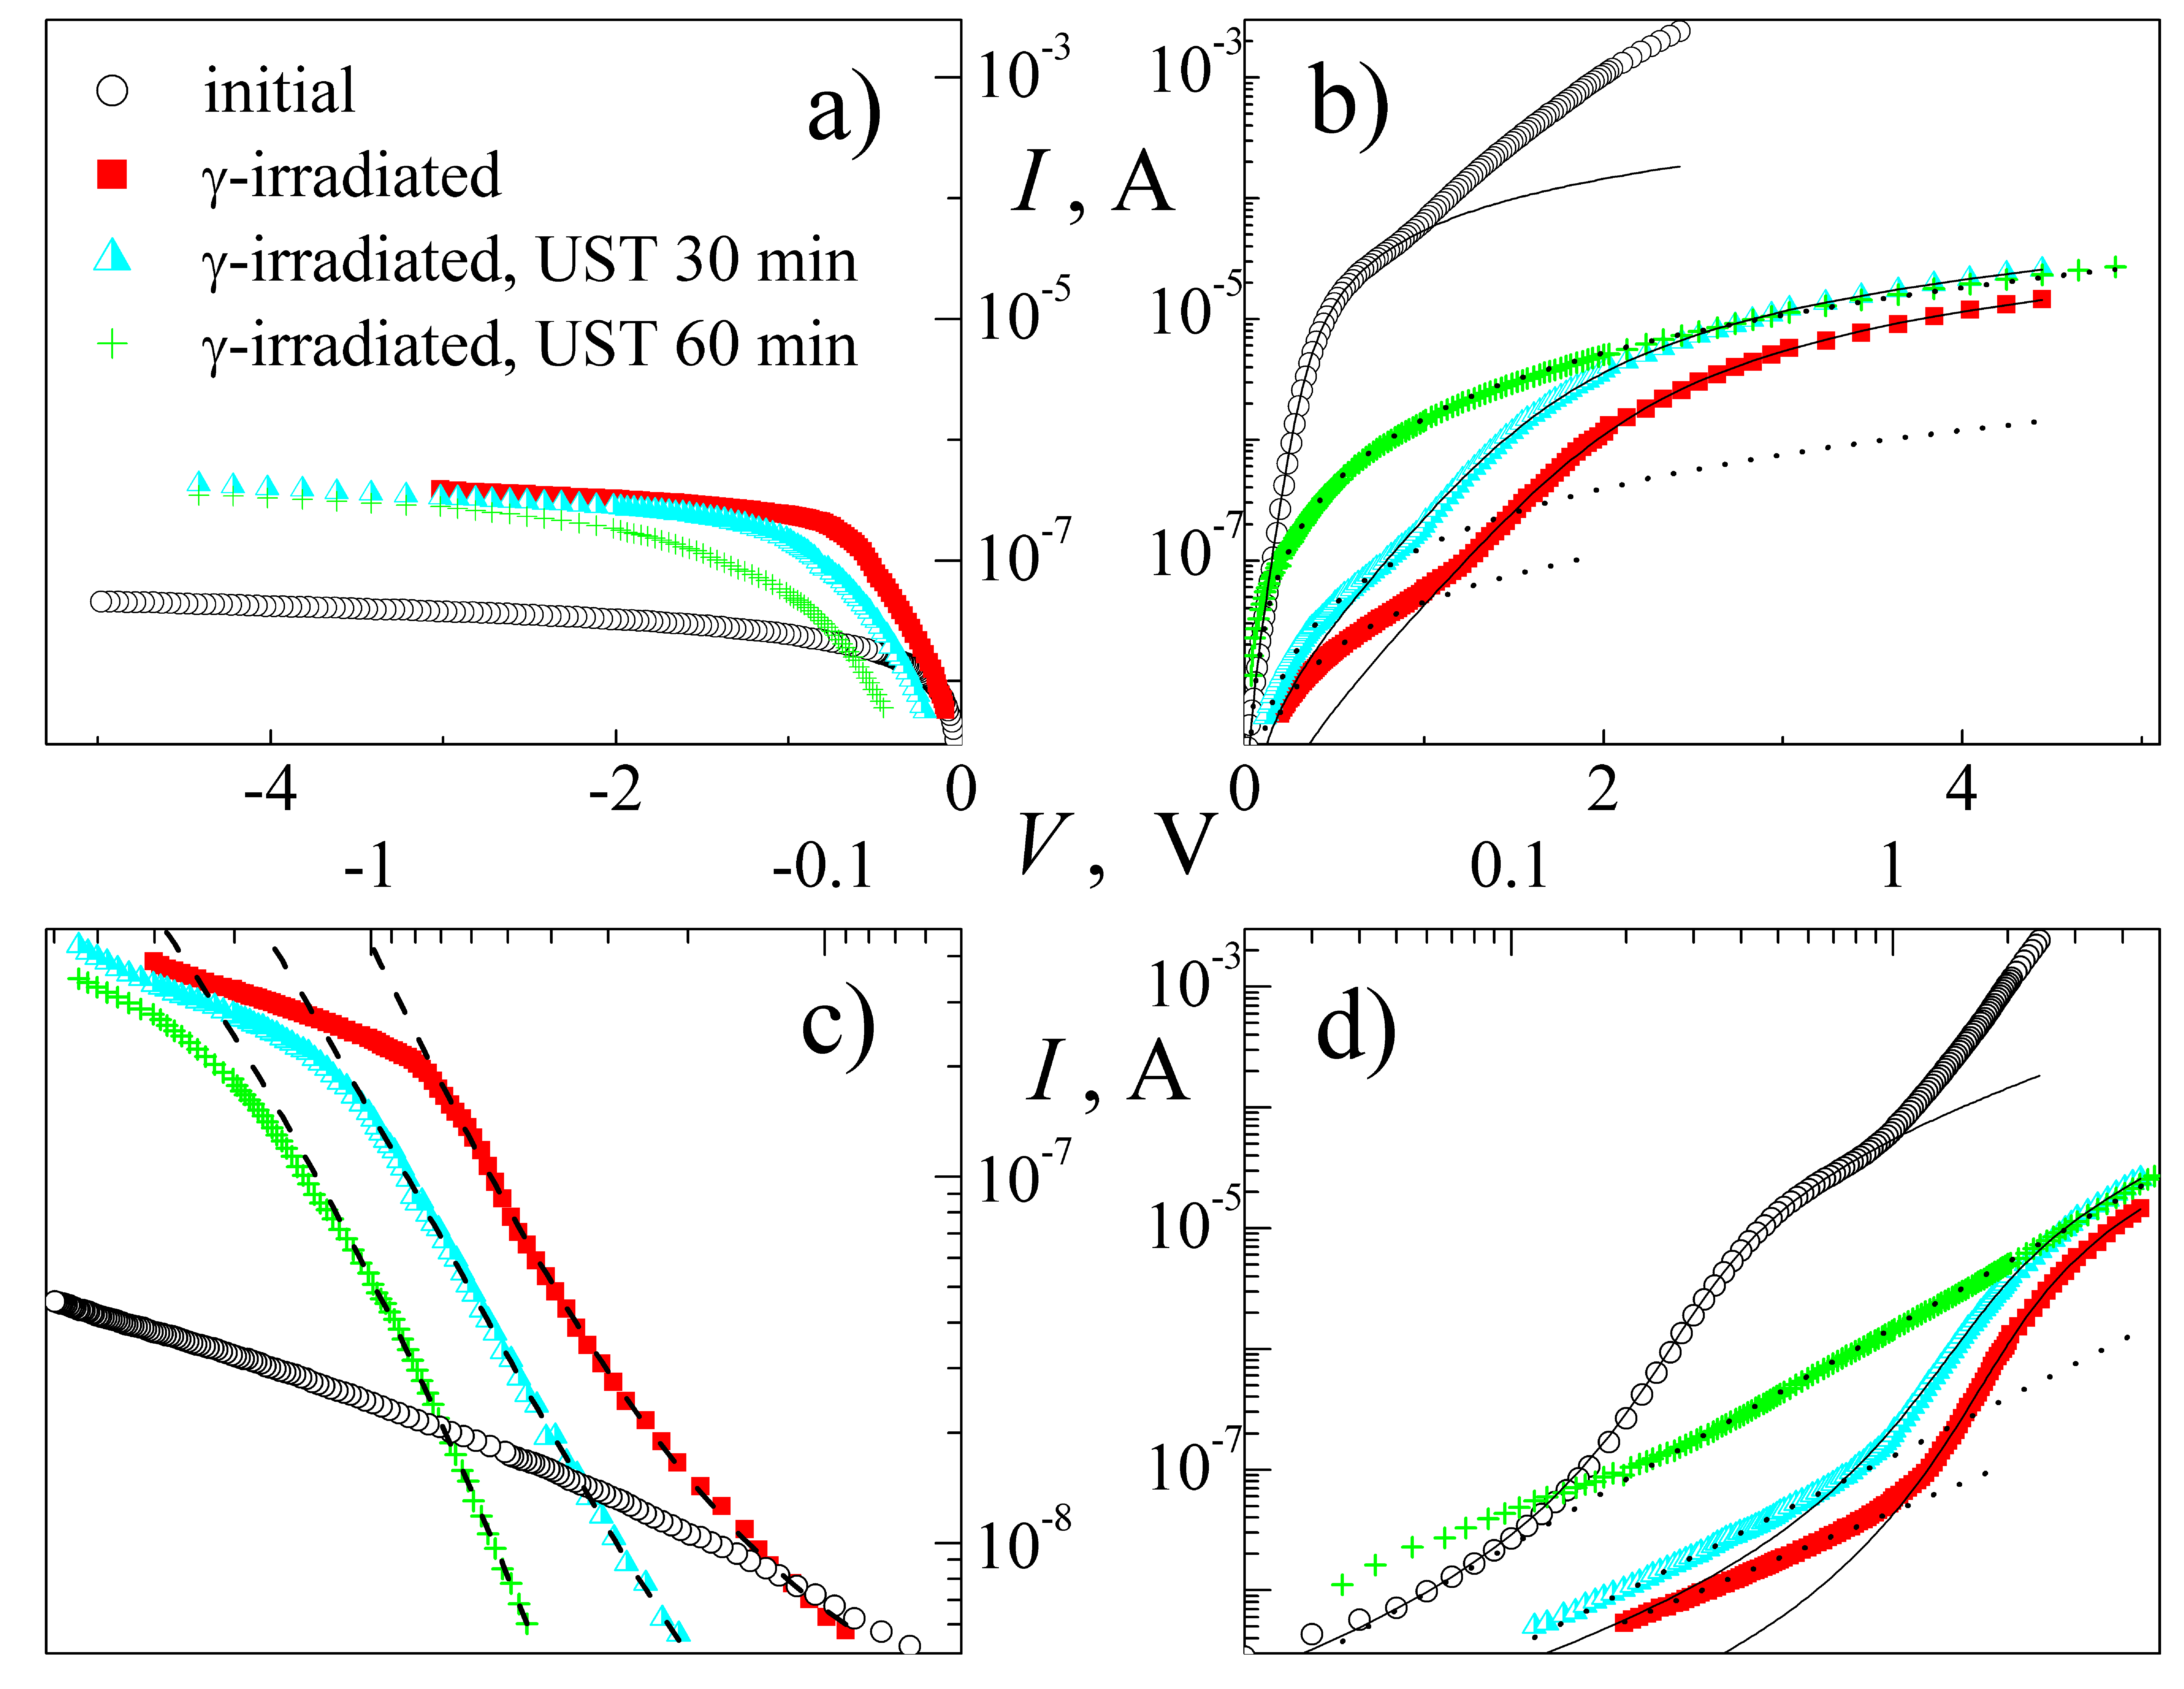
\includegraphics[width=0.95\textwidth]{figIV}}
\caption{\label{figIV}
The logarithmical (a, b) and double-logarithmical (c, d) plots of the reverse (a, c) and forward $I-V$ characteristics for Au--SiO$_2$--Si structure before and after $\gamma$--irradiation and UST.
$T=300$~K.
The marks are the experimental results,
and the solid, dashed, and dotted lines are the TE, TAT, and SCLC fitted curves using Eq.~(\ref{eqSDIV}), (\ref{eqIVTAT}), and (\ref{eqVIsclc}) correspondingly.
}%
\end{figure}




\begin{table}
\caption{\label{tabMIS}Extracted parameters for the Au--SiO$_2$--Si structure
}
\center
\begin{tabular}{lcccc}
\hline
\multicolumn{5}{l}{Structure status}\\\hline
$\gamma$--irradiation&$-$&$+$&$+$&$+$\\ 
UST&$-$&$-$&$+$&$+$\\ 
&&&30~min&60~min\\ \hline
\multicolumn{5}{l}{Parameter}\\\hline
$I_s$, $10^{-9}$A & 3.3& 1.1& 4.9& \\ 
$R_s$, $10^{4}$�� & 1.1& 13& 8.8& \\ 
$n$ & 1.7& 10.3& 9.9& \\ 
$m_\mathrm{F}$ & &1.3& 1.6& 1.8 \\ 
$I_0$, $10^{-8}$A & &$4.5$& $13$& $150$ \\ 
$I_{0,\mathrm{TAT}}$, a.u. & &1& 0.14& 0.04 \\ 
$U_d$, B & &0.73& 0.44& 0.12 \\ 
$R_\mathrm{TAT}$, a.u. & &1& 0.54& 0.33 \\ 
$K_\mathrm{RECT}$ ($V=0,5$~V)&770 &0.22& 1.33& 5.4 \\ 
\end{tabular}
\end{table}



\begin{figure}
\centerline{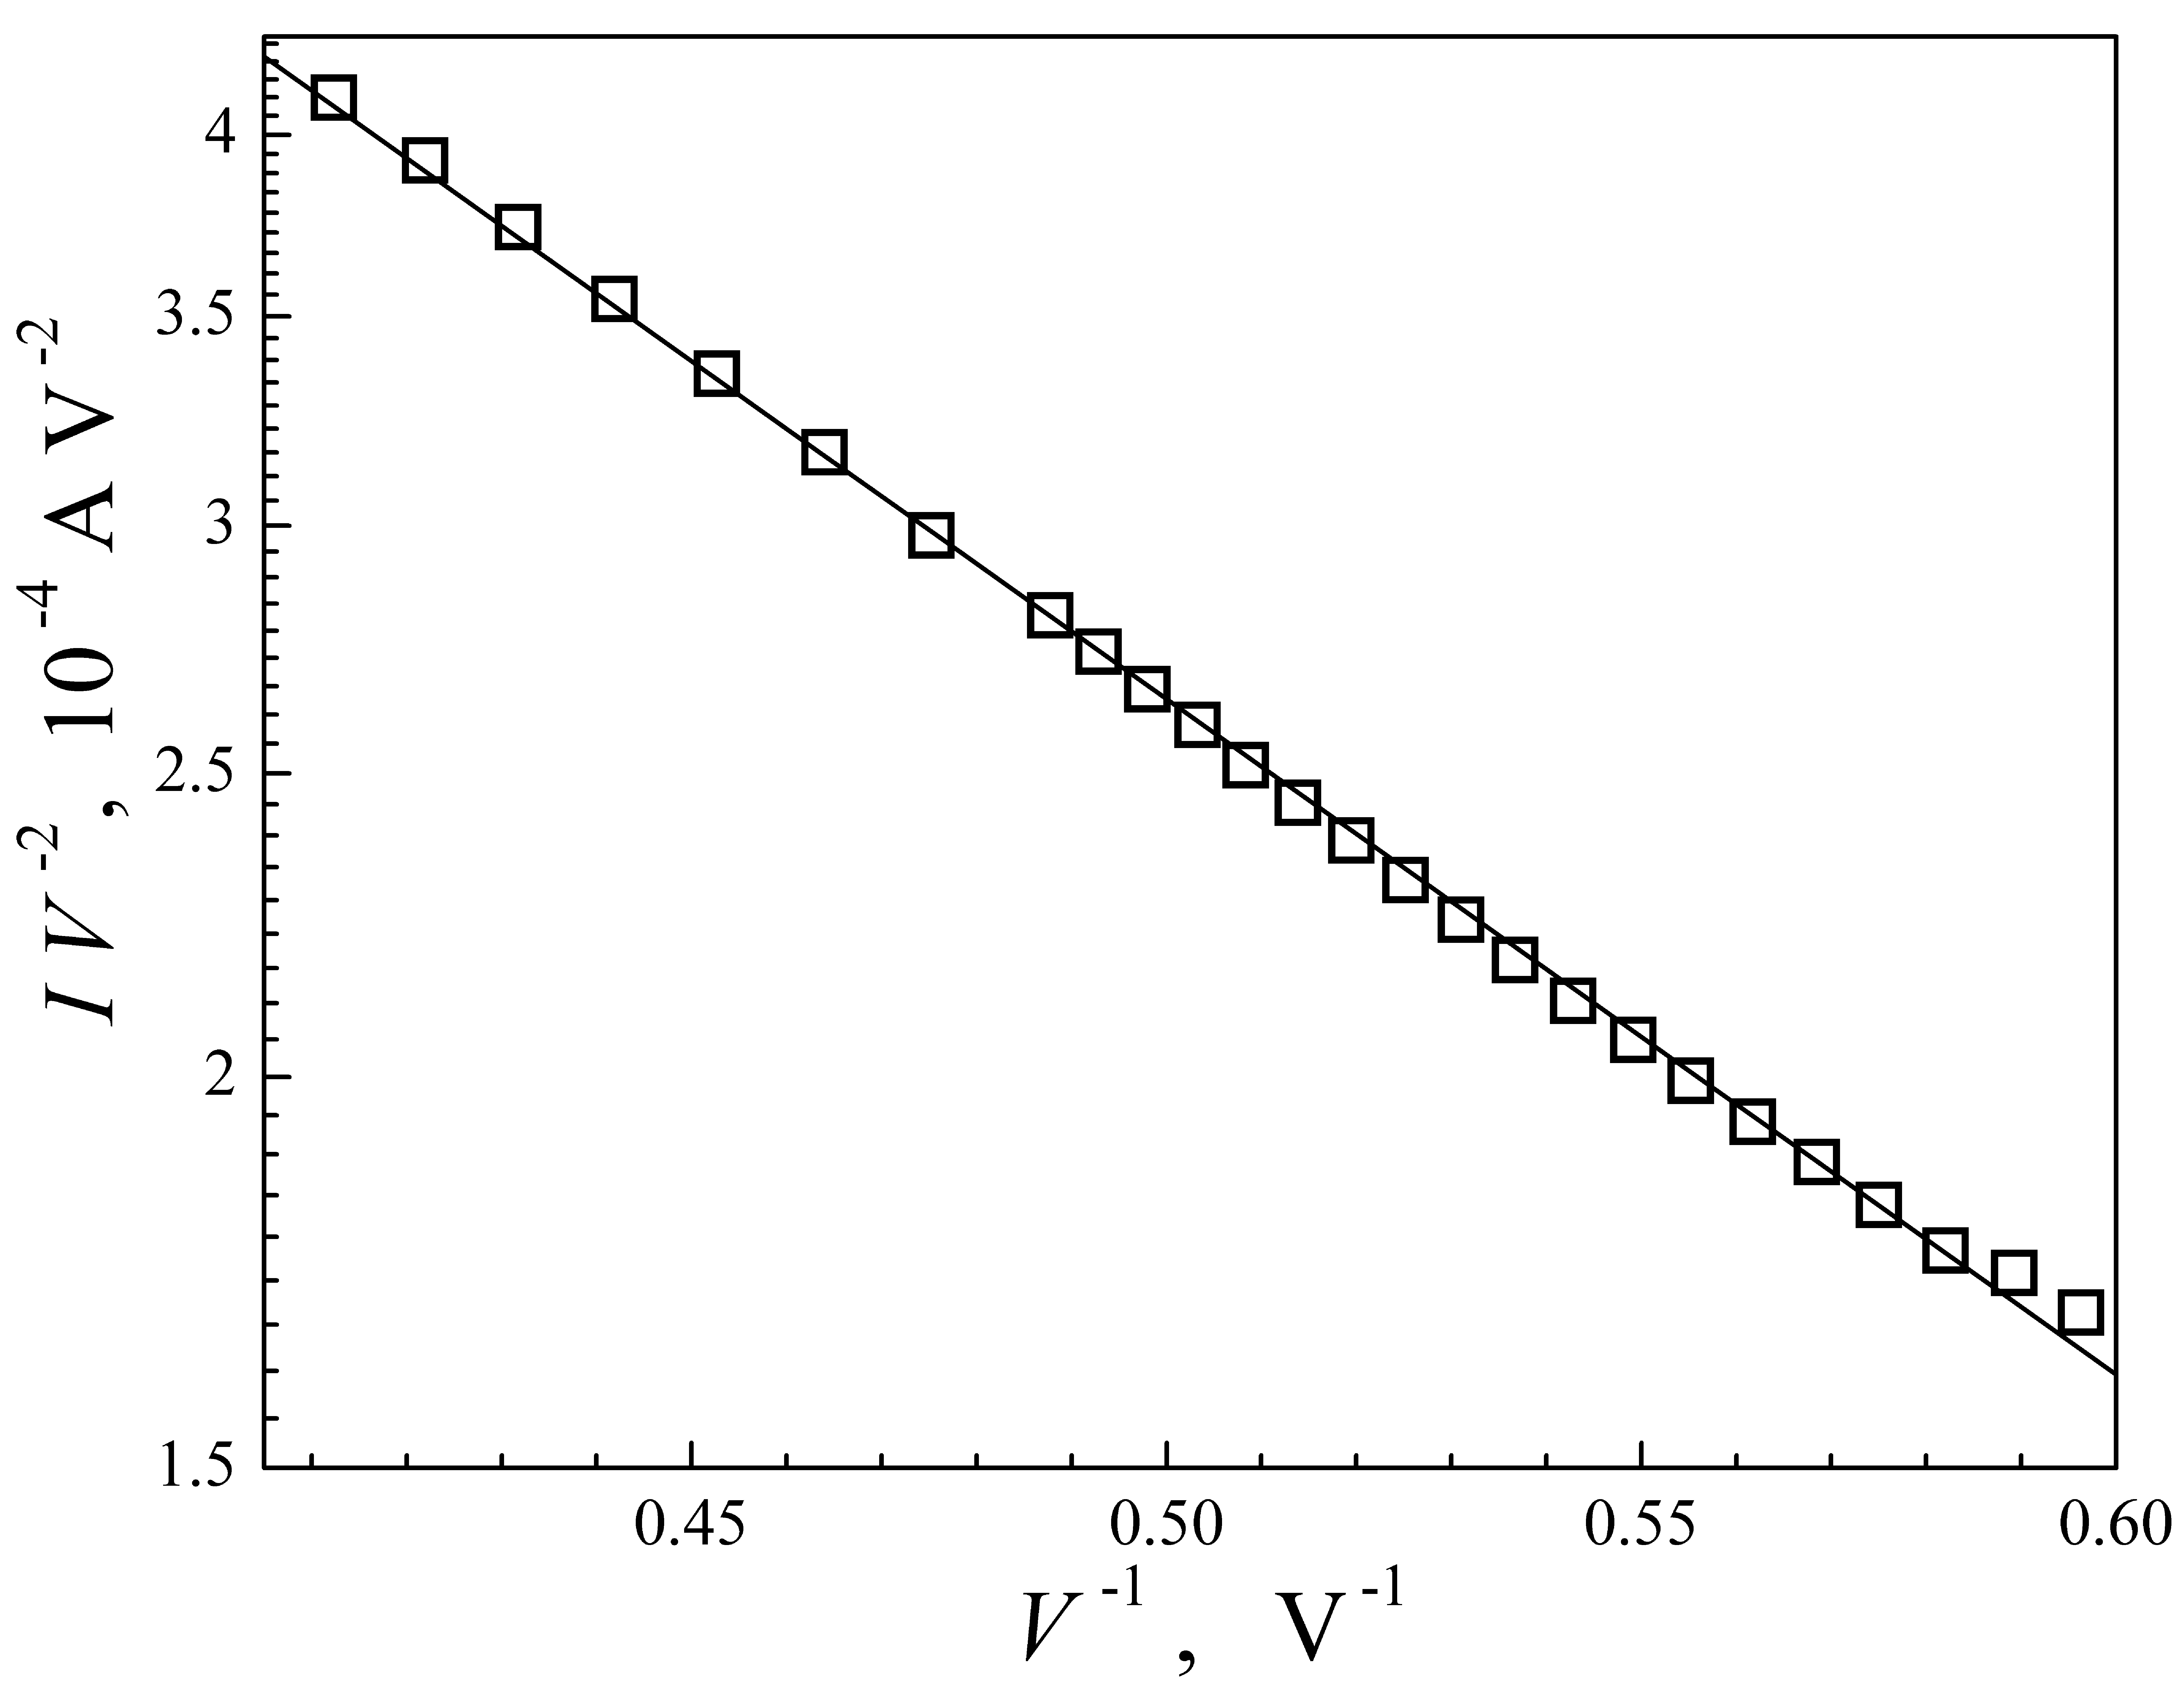
\includegraphics[width=0.6\textwidth]{FigFauler}}
\caption{\label{FigFauler}
The Fowler-Nordheim plot of the forward branch for non--irrradiated Au--SiO$_2$--Si structure at $V>1,6$~V.
The line is the least--squares linear fitting.
}%
\end{figure}



%The irradiation is known to lead to Si---H bond breakage at the Si--SiO$_2$ interface \cite{SiO2:Mahapatra,SiO2:Esseni}.

\begin{figure}
\centerline{
\includegraphics[width=0.6\textwidth]{figEa_MIS}}
\caption{\label{figEa_MIS}
Temperature dependence of SCLC--current for $\gamma$--irrradiated Au--SiO$_2$--Si structure before UST at $V=0,4$~V.
The line is the least--squares linear fitting.
}%
\end{figure}


%\section*{References}

\bibliography{olikh}

\end{document}

